\documentclass[11pt,letterpaper]{article}

\newenvironment{proof}{\noindent{\bf Proof:}}{\qed\bigskip}

\newtheorem{theorem}{Theorem}
\newtheorem{corollary}{Corollary}
\newtheorem{lemma}{Lemma} 
\newtheorem{claim}{Claim}
\newtheorem{fact}{Fact}
\newtheorem{definition}{Definition}
\newtheorem{assumption}{Assumption}
\newtheorem{observation}{Observation}
\newtheorem{example}{Example}
\newcommand{\qed}{\rule{7pt}{7pt}}

\newcommand{\solution}[4]{
\thispagestyle{plain} 
\newpage
\setcounter{page}{1}
\noindent
\begin{center}
\framebox{ \vbox{
\vspace{4mm}
\vspace{0.2in} 
{\centering \large\mbox{#3}}\\
\vspace{0.1in}
{#1 \hfill {Date: #2}}
}}
\end{center}
\markright{#1}
}

\newenvironment{algorithm}
{\begin{center}
\begin{tabular}{|l|}
\hline
\begin{minipage}{1in}
\begin{tabbing}
\quad\=\qquad\=\qquad\=\qquad\=\qquad\=\qquad\=\qquad\=\kill}
{\end{tabbing}
\end{minipage} \\
\hline
\end{tabular}
\end{center}}

\def\Comment#1{\textsf{\textsl{$\langle\!\langle$#1\/$\rangle\!\rangle$}}}



\usepackage{graphicx, amssymb, amsmath, listings, float, mathtools}
\usepackage{color, url}
\usepackage{romannum}
\lstset{language = Python}
\lstset{breaklines}
\lstset{extendedchars=false}
 
\definecolor{codegreen}{rgb}{0,0.6,0}
\definecolor{codegray}{rgb}{0.5,0.5,0.5}
\definecolor{codepurple}{rgb}{0.58,0,0.82}
\definecolor{backcolour}{rgb}{0.95,0.95,0.92}
 
\lstdefinestyle{mystyle}{
    backgroundcolor=\color{backcolour},   
    commentstyle=\color{codegreen},
    keywordstyle=\color{magenta},
    numberstyle=\tiny\color{codegray},
    stringstyle=\color{codepurple},
    basicstyle=\footnotesize,
    breakatwhitespace=false,         
    breaklines=true,                 
    captionpos=b,                    
    keepspaces=true,                 
    numbers=left,                    
    numbersep=5pt,                  
    showspaces=false,                
    showstringspaces=false,
    showtabs=false,                  
    tabsize=2
}
 
\lstset{style=mystyle}

\oddsidemargin 0in
\evensidemargin 0in
\textwidth 6.5in
\topmargin -0.6in
\textheight 9.0in

\begin{document}
% -----------------------------------------------------------------------------
\solution{\large Jifu Zhao}{\large 12/15/2016}{\bf \Large IE 529 \hspace{0.5cm} 
		Fall 2016 \hspace{0.5cm} Computational Assignment 2}

% -----------------------------------------------------------------------------
\section*{\Large \Romannum{1}. Lloyd's (K-means)Algorithm}

\begin{description}

\item{1. }
In this part, the polynomial regression is conducted on the given dataset. The derivation is relatively simple, here we only give one simple version.
 
\end{description}

% -----------------------------------------------------------------------------
\section*{\Large \Romannum{2}. Greedy K-centers Algorithm}

% -----------------------------------------------------------------------------
\section*{\Large \Romannum{3}. Single-Swap Algorithm}

% -----------------------------------------------------------------------------
\section*{\Large \Romannum{4}. Spectral Clustering Algorithm}

% -----------------------------------------------------------------------------
\section*{\Large \Romannum{5}. Expectation Maximization (EM) Algorithm}




\newpage
% -----------------------------------------------------------------------------
\begin{lstlisting}[language=Python, caption=Python example]

def polynomial_regression(x, y, degree, x_range):
    """ function to perform polynomial regression and compute least suares error
        
        Parameters:
        -----------
        x: input array, should have one dimension 
        y: fit goal, shoule have one dimension
        degree: polynomial degress
        
        return:
        -------
        w: weight matrix, the first value is intercept
        prediction: predicted values
        error: least squares error
    """
    
    n = len(x)
    # map x into multiple columns
    X = np.zeros((n, degree + 1))
    X[:, 0] = 1
    for i in range(1, degree + 1):
        X[:, i] = x ** i
    
    # reshape y into n by 1 format
    Y = np.array([y]).T
    
    # compute w, prediction and error
    w = np.dot(np.dot(np.linalg.inv(np.dot(X.T, X)), X.T), Y)
    error = np.sum((np.dot(X, w) - Y) ** 2)
    
    # compute the prediction
    new_X = np.zeros((len(x_range), degree + 1))
    new_X[:, 0] = 1
    for i in range(1, degree + 1):
        new_X[:, i] = x_range ** i
    prediction = np.dot(new_X, w)
    
    return w, error, prediction
\end{lstlisting}

% -----------------------------------------------------------------------------
%\begin{figure}[H]
%\centering
%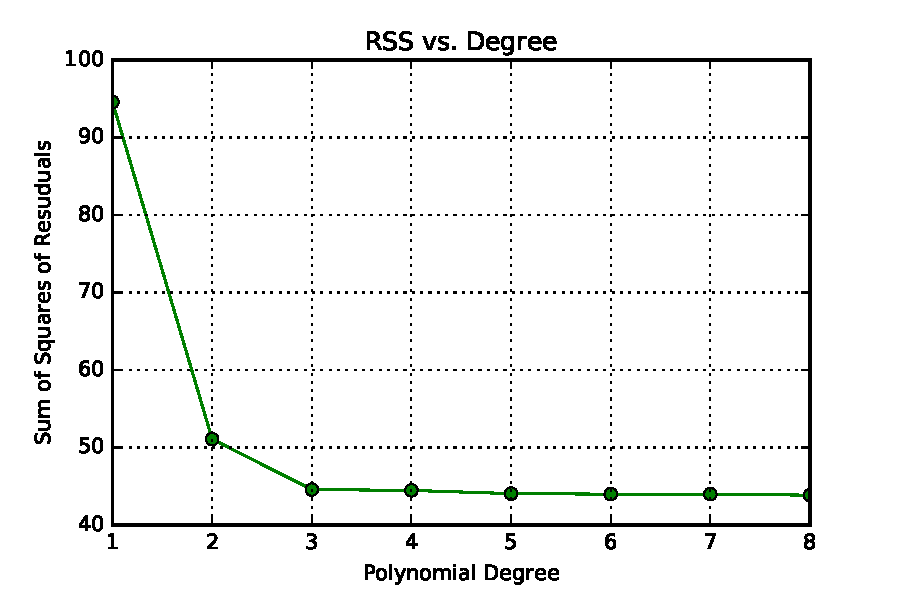
\includegraphics[width=0.9\textwidth]{./figures/rss.pdf}
%\caption{\label{fig:RSS} RSS for different models}
%\end{figure}


\clearpage

%\bibliographystyle{plain}
%\bibliographystyle{unsrt}
%\bibliography{reference.bib}

\end{document}

